\documentclass[a4paper,10pt]{report}
\usepackage[utf8]{inputenc}
\usepackage[english]{babel}
\usepackage{graphicx}
\usepackage{fancyhdr}
\usepackage{color}
\usepackage{url}

\topmargin 0pt
\advance \topmargin by -\headheight
\advance \topmargin by -\headsep
\textheight 8.9in
\oddsidemargin 0pt
\evensidemargin \oddsidemargin
\marginparwidth 0.5in
\textwidth 6.5in


\title{\huge{WSim tutorial for developers}}
\author{Loic Lemaitre}


\begin{document}
  \maketitle

\abstract{This document is aimed to help developers that would like to create or complement modules on WSim. It is not a full description of WSim source code, but a short introduction to allow to understand its architecture. It also gives some ways to debug your WSim code.}

  \tableofcontents

\chapter{Directories list}

WSim source code directory (\verb$/wsim$) contains the following subdirectories:
\begin{itemize}
  \item \verb$/arch$: implementation of the two supported MCU (MSP430 and ATMEGA).

  \item \verb$/autom4te.cache$:

  \item \verb$/devices$: implementation of external peripherals;

  \item \verb$/doc$: wsim website sources;

  \item \verb$/examples$: example codes to demonstrate WSim main features;

  \item \verb$/libconsole$: carries out the link with wconsole;

  \item \verb$/libelf$:

  \item \verb$/libetrace$: deals with the trace generation for eSimu;

  \item \verb$/libgdb$: carries out the link with the gdb debugger;

  \item \verb$/libgui$: used to show user interface (i.e. the leds blinking);

  \item \verb$/liblogger$: deals with error and output messages (wsim.log, error message on terminal);

  \item \verb$/libselect$: manages inputs and outputs between WSim and external application (WConsole, WSnet);

  \item \verb$/libtracer$: generates WSim traces (*.trc);

  \item \verb$/libwsnet$: carries out the link with WSnet;

  \item \verb$/machine$: make the link between platform model and simulator;

  \item \verb$/platforms$: implementation of the different platforms (wsn430, telosb, senslab...);

  \item \verb$/src$: point of entry of the program. Deal with the wsim options (arguments) too;

  \item \verb$/utils$: contains compilable sources of useful tools (WTracer, WConsole, ...);
\end{itemize}


\chapter{Program execution overview}
\label{prog-exec}

The point of entry of the program is the \verb$main.c$ file located in the \verb$src/$ directory. The program starts by adding base options and specific options of the platform.
Simulation steps:

\begin{figure}[ht]
\begin{center}
 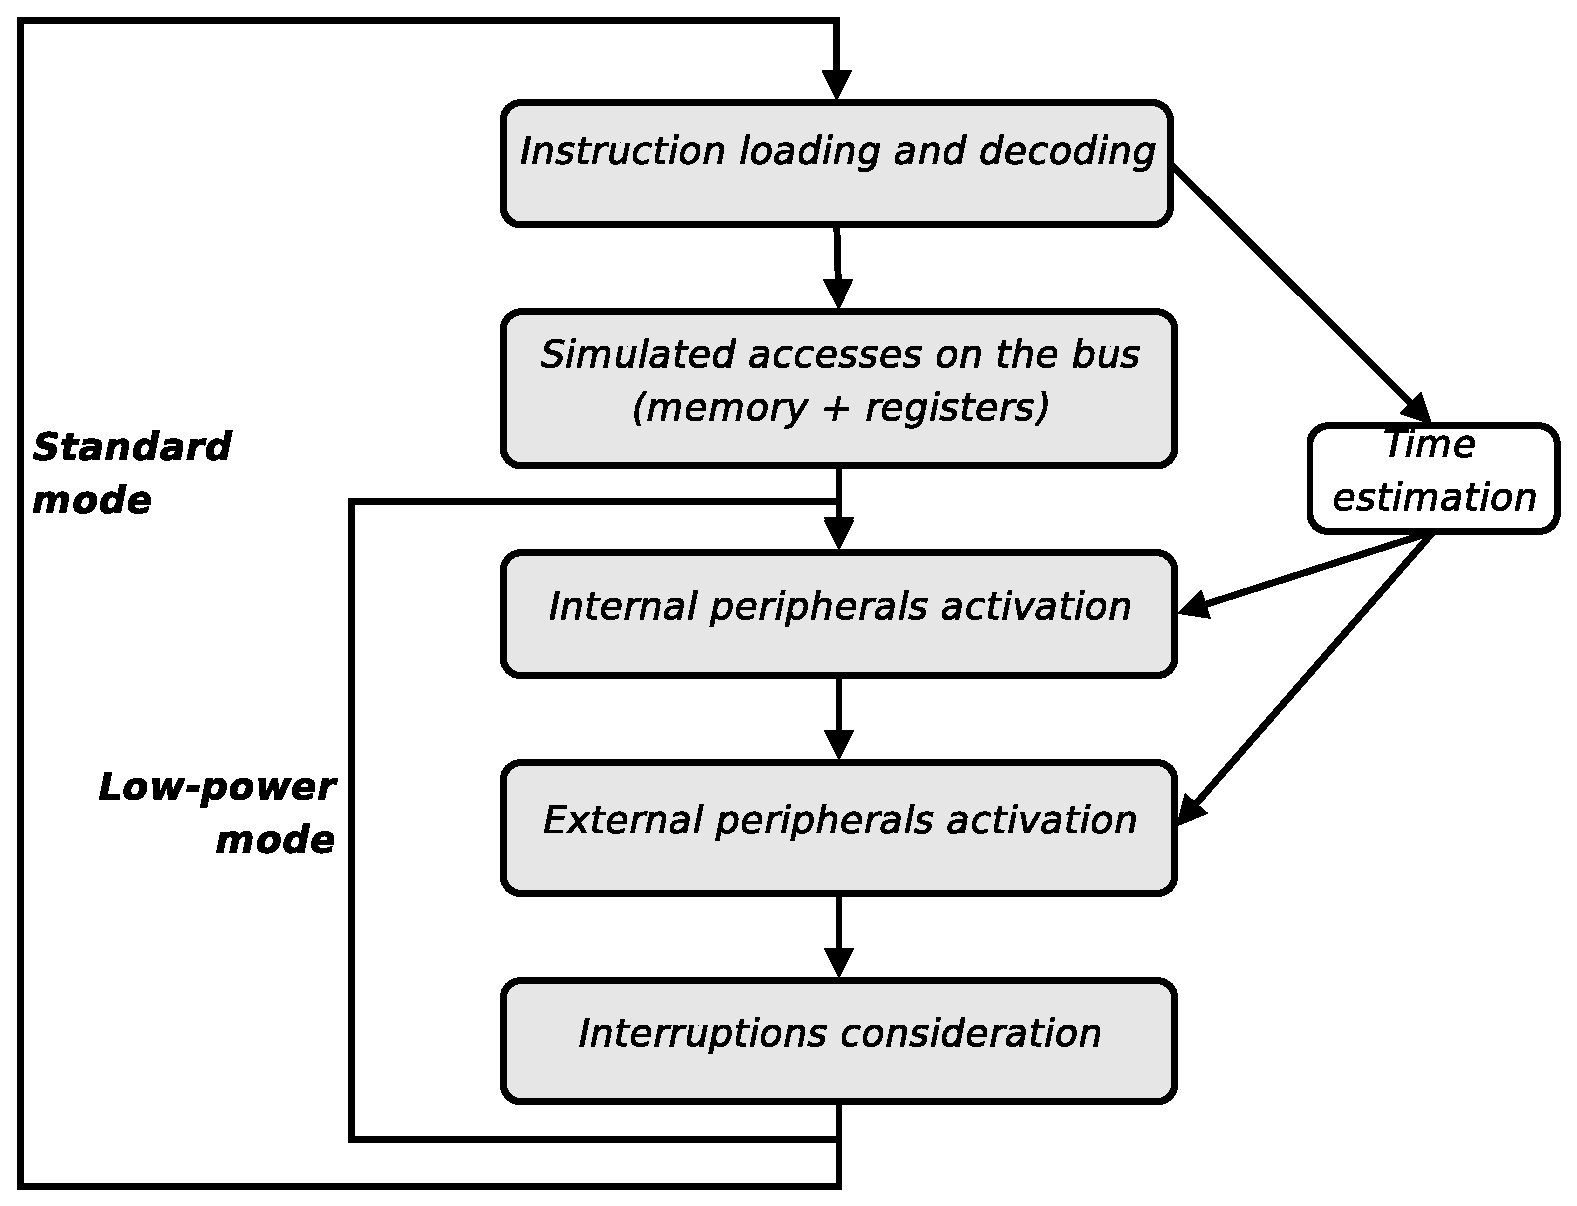
\includegraphics[scale=0.4]{figures/wsim_diag.eps}
\end{center}
\caption{WSim execution diagram}
\label{wsim diagram}
\end{figure}


\chapter{Main internal features management}

\section{Memory}
\subsection{General}
Main storages are MCU state, platform external devices state (radio, leds, ...), and possibly internal platform state. A backup of these states is periodically carried out so that it allows to recover easily the previous saved state of the platform in order to backtrack.

\subsubsection{Devices and platform}
When a platform is built, an instance of each of its devices is created in order to save its states. The memory allocation  is done by the \verb$devices_memory_allocate()$ function of the \verb$devices.c$ file, located in the \verb$/devices$ directory. This function is called by the platform description file. In this function, the needed space to save the states of every platform device is computed, in order to store all the data in a contiguous memory spaces.  The pointers to access to them are stored into the \verb$machine.devices_state$ and the \verb$machine.devices_state_backup$ (\verb$machine$ is a global structure storing devices states, devices number, devices size and time of simulation).\\

Moreover saving internal platform states may be necessary. They are then stored in a platform specific structure (of your platform file), you have to define. This structure must be saved in the same contiguous space than the devices, by considering it as a device.

\subsubsection{MCU}
The MCU state and its backup are stored into global structures (\verb$mcu$ and \verb$mcu_backup$), since we know the needed space and as there is only one MCU by platform. So we need not indirections (through pointers) to access to the MCU structure, in spite of the device structure.

\subsection{Backtracks}
Backtracks are used when WSim operates with WSnet. Indeed WSim may need to backtrack in two different cases:
\begin{itemize}
  \item when one of WSim nodes runs beyond a meeting point, since nodes synchronisation is done by an appointment method. An other meeting point is then set, and the state of the node is restored to the last state saved;
  \item when one of WSim nodes is in debugging mode, and stopped at a breakpoint, the other nodes are still running. As soon as the WSim node in debugging mode is running again, the other nodes are backtracked.
\end{itemize}

\begin{figure}
\begin{center}
  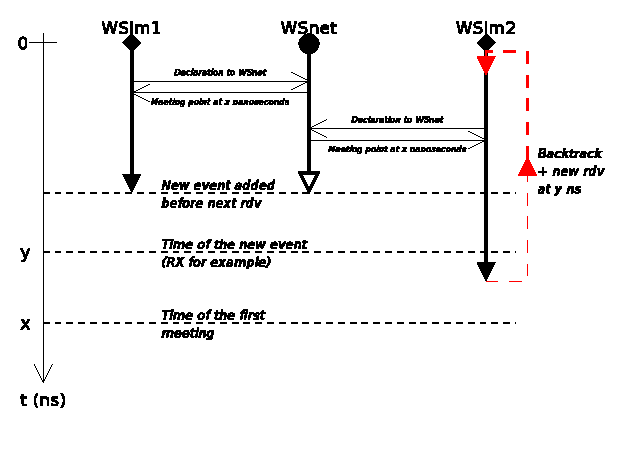
\includegraphics[scale=1]{figures/wsim_backtrack1.eps}
\end{center}
\caption{WSim backtrack when a node runs beyond a meeting point}
\label{wsim backtrack 1}
\end{figure}

\begin{figure}
\begin{center}
  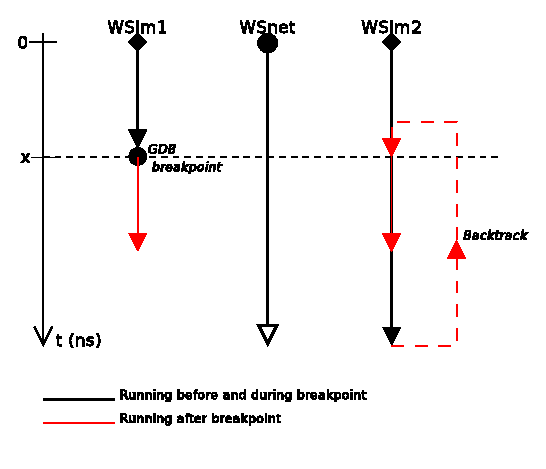
\includegraphics[scale=1]{figures/wsim_backtrack2.eps}
\end{center}
\caption{WSim backtrack in debugging mode}
\label{wsim backtrack 2}
\end{figure}

State backup saves are performed by WSim nodes through the \verb$void machine_state_save()$ function, as soon as a synchronisation is successfull or a response is received by WSnet from a WSim node. To come back from the present state to the backup one, \verb$void machine_state_restore()$ of the \verb$/machine/machine.c$ file is called. This function executes the following tasks:
\begin{itemize}
  \item restoring the state of the MCU (copy of the MCU structure in the MCU backup structure)
  \item setting the time simulation to the time of the backup
  \item replacing the content of the present state memory by the content of the backup state one
  \item restoring traces
  \item restoring WSnet state
\end{itemize}

\section{Signals}
\verb$/arch/common/mcu.h$

\section{I/O}
\verb$/libselect$


\chapter{Implementing new WSim modules}

\section{Platform}
In the WSim design, the platform file is aimed to describe it, but also to make a link between MCU and devices.
\subsection{Implementing your platform}
\subsubsection{Headers to include}
You have to include the following files in your platform implementation:
\begin{itemize}
  \item The MCU common header (\verb$#include "arch/common/hardware.h"$) and the MCU specific header (\verb$#include "arch/msp430/msp430.h"$ or \verb$#include "arch/atmega/atmega128.h"$);
  \item The device common header (\verb$#include "devices/devices.h"$) and the header of each implemented devices of the platform;
  \item \verb$#include "src/options.h"$ if you want to add platform specific options.
\end{itemize}

\subsubsection{List of mandatory functions to implement}
\begin{itemize}
  \item \verb$int devices_options_add(void)$: adds platform specific options with the \verb$option_add()$ function;
  \item \verb$int devices_create(void)$: computes the needed memory space for devices and initialise them;
  \item \verb$int devices_reset_post(void)$: function called after devices reset, so devices init conditions must be written here;	
  \item \verb$int devices_update(void)$: function called after every MCU instruction execution, this function handles input and output between MCU and devices ports.
\end{itemize}

\subsubsection{Intructions in devices\_create() function}
This function is called only once at the simulation initialisation. This intructions sequence should be followed:
\begin{enumerate}
  \item You have first to take into consideration potential specific options, that might have been provided as a command line argument (only if you implement specific option in \verb$devices_option_add()$). This is done by checking the \verb$value$ item of each option structure.
  \item MCU must be initialised by calling its \verb$MCUNAME_create()$ function;
  \item Fix each device size and store it in the \verb$machine.device_size$ table. Now \verb$devices_memory_allocate()$;
  \item Create each device with its \verb$DEVICENAME_device_create()$ function;
  \item Initialise UIs by getting their sizes (\verb$machine.device[DEVICEID].ui_get_id()$) and set their positions (\verb$machine.device[DEVICEID].ui_set_pos()$).
\end{enumerate}

\subsubsection{Intructions in devices\_update() function}
This function is the core of the platform because it describes GPIO and SPI connections between MCU and . Thus every time the MCU decodes an intruction, this function will be called.
Instructions sequence is important and you have to follow this order as explained previously (cf chapter \ref{prog-exec} page \pageref{prog-exec}): MCU to devices transfer, devices to MCU transfer, devices update. Otherwise SPI communications might experience dysfunctions.

\begin{enumerate}
  \item First you begin by reading the MCU pins with this function: \verb$MCUNAME_digiIO_dev_read()$, that reads the 8 pins of a MCU port. Then depending of the devices pins configuration, transfer the received value on the right devices pins, by using \verb$machine.device[DEVICEID].write()$. Reiterate the sequence as many times as the number of MCU ports;
  \item Do the same operation with the UART or/and SPI ports: use \verb$msp430_UARTORSPI+ID_dev_read_$\linebreak\verb$UARTORSPI()$ to get pins value and \verb$machine.device[DEVICEID].write()$ to send it to the connected device;
  \item Now repeat the two first steps in the opposite direction, that is to say from devices to MCU pins. Use  \verb$machine.device[DEVICEID].read()$ to read devices pins and \verb$msp430_usart+ID_dev_write_$\linebreak\verb$UARTORSPI()$ to write MCU SPI or UART pins, or \verb$msp430_digiIO_dev_write()$ to write MCU GPIOs.
  \item Finally these modules must be updated:
  \begin{description}
    \item -libselect to update external I/O of WSim: \verb$LIBSELECT_UPDATE()$;
    \item -libwsnet to update link with WSnet : \verb$LIBWSNET_UPDATE()$;
    \item -platform devices to update their internal states: \verb$machine.device[DEVICEID].update()$ for each device.
  \end{description}
\end{enumerate}

\noindent\underline{Remark:} To make your platform more reliable, and give value-added to the simulation, you may add tests for illegal operations not to happen, for example:
\begin{itemize}
  \item Checking if MCU is in SPI mode before reading a SPI device;
  \item Checking if MCU is in UART mode before reading an UART device;
  \item If there are more than one device on one SPI, checking that their CSs are not enabled at the same time;
  \item Any other test you need...
\end{itemize}


\subsubsection{SDL/UI - Input}
UI is considered as a device


\subsection{Making your platform executable}
To compile WSim, makefiles are generated with the help of the GNU Project Autotools (automake $\ge$ 1.10, autoconf $\ge$ 2.61) \footnote{For further information please see http://www.gnu.org/software/automake/ and 
http://www.gnu.org/software/autoconf/ websites}.


\section{Device}
\subsection{Adding a new device model}
\subsubsection{List of mandatory functions to implement}
\begin{itemize}
  \item \verb$int DEVICENAME_add_options()$: enables to add device specific options when starting a simulation.
  \item \verb$int DEVICENAME_device_size()$: returns size the device structure needs to store its internal states.
  \item \verb$int DEVICENAME_device_create()$: creates an instance of the device, by initialising the states in \verb$machine.device[DEVICEID].data$ and storing in \verb$machine.device[DEVICEID]$ device private functions to be called during the simulation.
\end{itemize}

\subsubsection{List of optional functions to implement}
Depending of devices features some of these private functions have to be implemented:
\begin{itemize}
  \item \verb$int DEVICENAME_write()$: transmits MCU informations to the device
  \item \verb$int DEVICENAME_read()$: transmits device informations to the MCU (for example leds need not this function);
  \item \verb$int DEVICENAME_update()$: updates internal state of the device after read or write action (for instance emptying radio TX buffer after its content has been transmitted to the MCU);
  \item \verb$int DEVICENAME_delete()$: frees memory space filled by the device (excepted the device states);
  \item \verb$int DEVICENAME_reset()$: resets the device (at its default states);
  \item \verb$int DEVICENAME_power_up()$: for potential futur use;
  \item \verb$int DEVICENAME_power_down()$: for potential futur use;
  \item \verb$int DEVICENAME_ui_draw()$: draws device graphical interface;
  \item \verb$int DEVICENAME_ui_set_pos()$: sets the position of device graphical interface;
  \item \verb$int DEVICENAME_ui_get_pos()$: gives the position of device graphical interface;
  \item \verb$int DEVICENAME_ui_get_size()$: gives the size of device graphical interface;
  \item \verb$int DEVICENAME_statdump()$: may be used to return device statistics (only called at the end of the simulation).
\end{itemize}

\subsection{GPIO interface management}

\subsection{SPI interface management}
\subsubsection{General}
The SPI interface is implemented in the file \verb$arch/msp430/msp430_usart.c$ for the MSP430 MCU.

\subsubsection{Particular case}
Although WSim tries to be as close as possible to hardware it simulates, it may remain some differences. That is sometimes the case of the SPI and device communication simulation, depending of the device implementation.\\

In effect when a byte is written in the SPI UxTXBUF register, this one is sent bit by bit to the SPI linked device, and simultaneously this one replies bit by bit to the UxRXBUF register. Similarly, a dummy byte must be written in the UxTXBUF in order to read data from a SPI device.\\

Concerning WSim, in the platform description file, the following order must be respected in the \verb$device_update()$ function, as explained previously: write device from MCU, read device from MCU, update device.
Now, for some devices (cc2420, cc1100, ...), writing on their SPI input (SI) is taken into consideration only when the device is updated at the end of a cycle. As the read action is performed after the write one, no response is sent on the device SPI output (SO) yet.\\

This leads to a small lag between the simulation and the reality, since the SPI UxRXBUF register receives the response on the next \verb$device_update()$ call, that is to say few MCU cycles later (from 1 to 6).
The figure~\ref{wsim spi communication} illustrates that.\\

\begin{figure}[!h]
\begin{center}
  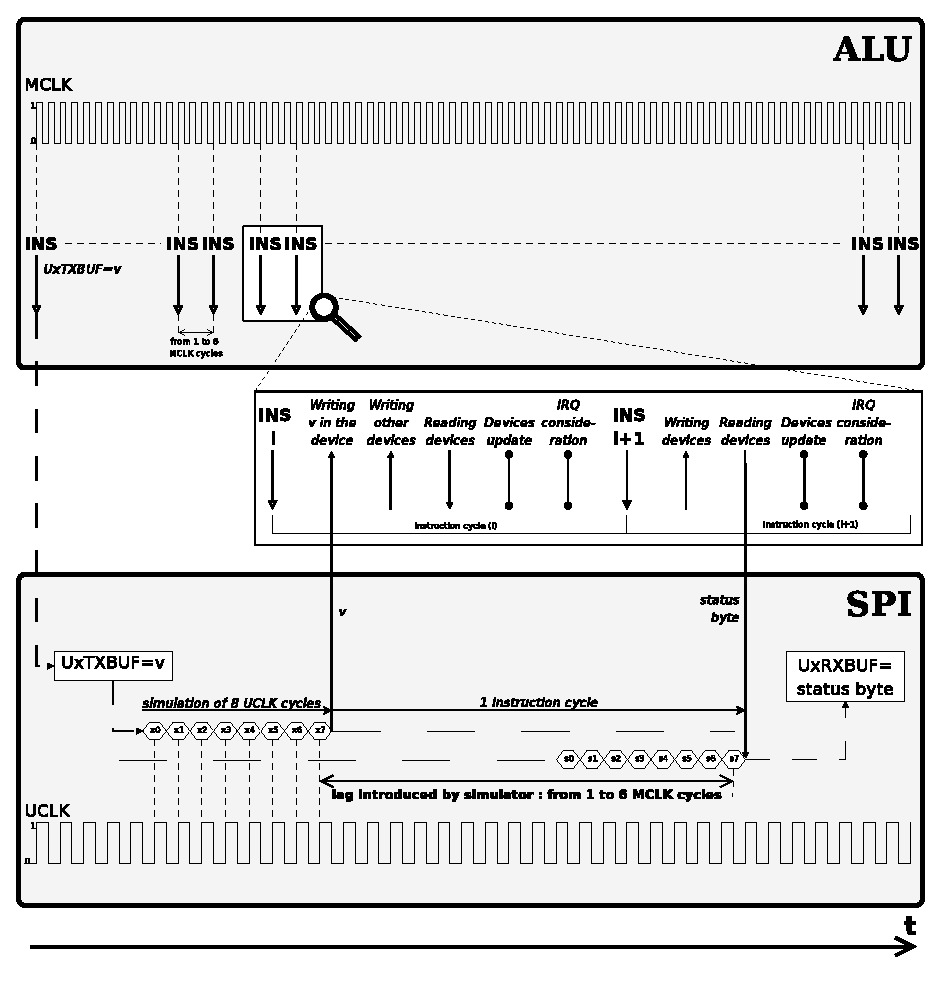
\includegraphics[scale=1]{figures/wsim_spi.eps}
\end{center}
\caption{WSim SPI and device communication particular case}
\label{wsim spi communication}
\end{figure}

In most cases this small lag will not be annoying. But if you want to avoid or fix it, you have to write or correct the device model, so that writing and reading on SPI ports trigger immediately an update.


\subsection{I2C}
Not implemented yet!

\section{Special device}
\subsection{Pseudo serial PTTY}


\section{Microcontroller}


\chapter{Debugging WSim}

There are several methods to debug WSim code source.

\section{wsim.log file}

At each simulation a log file is generated by WSim, named wsim.log and located in the directory where WSim has been launched. This file contains debugging information.
To enable debugging information, you have to define the macro DEBUG. There are two ways to do so:

\begin{itemize}
  \item when launching \verb$configure$ file before compiling WSim add the option \verb$./configure --enable-debug$;
  \item or define directly the macro \verb$DEBUG$ in the WSim file \verb$xxx_debug.h$ located in the same directory than the file you want to debug, as shown in the following example:
\end{itemize}

\begin{verbatim}
/**
 *  \file   cc2420_debug.h
 *  \brief  CC2420 debug messages 
 *  \author Nicolas Boulicault
 *  \date   2007
 **/

/*
 *  cc1100_debug.h
 *  
 *
 *  Created by Nicolas Boulicault on 04/06/07.
 *  Copyright 2007 __WorldSens__. All rights reserved.
 *
 */

#ifndef _CC2420_DEBUG_H_
#define _CC2420_DEBUG_H_

/***************************************************/
/***************************************************/
/***************************************************/

#define DEBUG
#if defined(DEBUG)
#define CC2420_DEBUG(x...)     VERBOSE(2,x)
#define CC2420_DBG_RX(x...)    VERBOSE(2,x)
#define CC2420_DBG_TX(x...)    VERBOSE(2,x)
#else
#define CC2420_DEBUG(x...)     do { } while (0)
#define CC2420_DBG_RX(x...)    do { } while (0)
#define CC2420_DBG_TX(x...)    do { } while (0)
#endif

/***************************************************/
/***************************************************/
/***************************************************/

#define CC2420_PINS_DEBUG

\end{verbatim}

The second method has the advantage to print only debug messages of the file where \verb$DEBUG$ is defined, contrary to the first one that behaves like \verb$DEBUG$ were defined in each file of the program.

By default, debugging information in wsim.log file is minimal.(default verbose level equal to 0). Nevertheless more information may be output be increasing verbose level when starting simulation: \verb$--verbose=6$ for instance.
In the previous code, we have \verb$#define CC2420_DBG_RX(x...)    VERBOSE(2,x)$. This means that the \verb$CC2420_DBG_RX$ will be print in the wsim.log file only if the verbose level is superior or equal to 2.

Thus you understand that it is quite easy to add your own debug informations, if you need. You just have to define the print debugging function with its verbose level at the beginning of your file (or its associated *.h file). Then insert it with appropriate debugging message (a \verb$printf()$ function) at the right place.

Notice that the \verb$wsim.log$ file name may be changed into \verb$NAMEOFYOURCHOICE.log$ by using the option \verb$--logfile=NAMEOFYOURCHOICE.log$.

\section{The ERROR() function}
The \verb$ERROR()$ function is closed to the \verb$VERBOSE()$ function, excepted that its result is printed in the wsim.log file and in the standard error output too, that is to say the terminal you launch WSim.
You can insert \verb$ERROR()$ function where you want without needs to declare it. Its syntax is as a \verb$printf()$ function.
Moreover some ERROR messages are printed only if the macro \verb$DEBUG_ME_HARDER$ is defined:
\begin{verbatim}
#if defined(DEBUG_ME_HARDER)
	    ERROR("senslab:devices: read data on radio while not in SPI mode ?\n");
#endif
\end{verbatim}

\section{Wsim trace}
The \verb$tracer_event_record()$ function, insered in the Wsim code, allows to save states of a variable during the simulation. To enable the trace storage, you just have to add the following option when starting a simulation: \verb$--trace$ (example: \verb$wsim-wsn430 --ui --trace --mode=time --modearg=100000000000$ \verb$wsn430-leds.elf$). The trace is then stored in the \verb$wsim.trc$ file and located in the  directory where WSim has been launched.

To make the wsim.trc file usable, you have to convert it with the external wtracer application, according to the following syntax. For instance:
\begin{itemize}
  \item\verb$wtracer --in=wsim.trc --out=wsim.gp --format=gplot$ gererates the gnuplot wsim.gp file. 
  \item\verb$wtracer --in=wsim.trc --out=wsim.vcd --format=vcd$ gererates the vcd wsim.vcd file, readable by GTKwave.
\end{itemize}


\section{Using GDB}
It is also possible to debug WSim by using GDB. Launch GDB in the folder where the *.elf file is located, set your breakpoints, and execute the run command followed by the WSim arguments, including your *.elf file. Here is an example:
\begin{verbatim}
loic@loic-laptop:~/Documents/Senstools/temp/senslab/node/wsn430_SW/wsn430-drivers/
wsn430-cc2420\$ gdb wsim-senslabv14
GNU gdb 6.8-debian
Copyright (C) 2008 Free Software Foundation, Inc.
License GPLv3+: GNU GPL version 3 or later <http://gnu.org/licenses/gpl.html>
This is free software: you are free to change and redistribute it.
There is NO WARRANTY, to the extent permitted by law.  Type "show copying"
and "show warranty" for details.
This GDB was configured as "i486-linux-gnu"...
(gdb) b main.c:200
Breakpoint 1 at 0x8054568: file main.c, line 200.
(gdb) r cc2420-tx.elf 
Starting program: /usr/local/bin/wsim-senslabv14 cc2420-tx.elf
[Thread debugging using libthread_db enabled]
[New Thread 0xb7c168c0 (LWP 23589)]
[Switching to Thread 0xb7c168c0 (LWP 23589)]

Breakpoint 1, main (argc=2, argv=0xbf976f24) at main.c:200
200	  options_start();
(gdb) n
201	  ui_options_add();
(gdb) 
\end{verbatim}


\chapter{Appendix}

\section{Abbreviations}
\begin{description}
  \item CS = Chip Select
  \item GPIO = General Purpose Input Output
  \item I2C = Inter Integrated Circuit
  \item MCU = MicroController Unit
  \item PTTY =
  \item SI = SPI device input
  \item SO = SPI device output
  \item SPI = Serial Peripheral Interface
  \item UART = Universal Asynchronous Receiver Transmitter
  \item UI = User Interface
  \item USART = Universal Synchronous/Asynchronous Receiver Transmitter
  \item UxRXBUF = SPI register used for reception
  \item UxTXBUF = SPI register used for transmission
\end{description}



\end{document}          
